\documentclass{beamer}
\usetheme{Boadilla}
\usepackage[english]{babel}
%\usepackage{beamerthemesplit}
\usepackage{amsmath}
\usepackage{graphicx}
\usepackage{wrapfig}
\usepackage{color}
\usepackage{setspace}
\usepackage{multicol}
\setbeamertemplate{frametitle}{ \bf
\begin{centering} 
\insertframetitle 
\par 
\end{centering} 
} 

\newcommand\Fontvi{\fontsize{9}{9}\selectfont}
\newcommand\Fontvii{\fontsize{4}{4}\selectfont}
\newcommand\Fontv{\fontsize{11}{11}\selectfont}
\newcommand\Fontb{\fontsize{20}{20}\selectfont}
\newcommand\Fontsm{\fontsize{13}{13}\selectfont}


\title[Superconducting Susceptibility]{Electronic Spin Susceptibility Enhancement in Pauli-Limited Superconductors}
\author[brosemeyer@physics.montana.edu]{Ben Rosemeyer \\ \small Advisor: Anton Vorontsov}
\institute[MSU]{
\includegraphics[scale=0.2]{MSUlogo.jpg}\\[0.5cm]
Funded by NSF grant DMR-0954342 \\
\includegraphics[scale=0.08]{NSFlogo.jpg}
}
\date[APS March Meeting 2013]{\small\today}



\begin{document}
\frame{\titlepage}

%\section*{Outline}
%\frame{\tableofcontents}


\begin{frame}
\frametitle{Motivation}
\centering
\colorbox{purple}{\textcolor{yellow}{Superconductivity and Magnetism}} \\ \vspace{0.2cm}
\quad \quad-Pnictides (LaOFeAs and BaFe$_2$As$_2$ groups) \\ \vspace{0.2cm}
\quad -Triplet superconducters ((TMTSF)$_2$PF$_6$, Bechgaard Salts)\\ \vspace{0.2cm}
\quad -High $T_c$ cuprates (Ba$_2$Ca$_4$Cu$_5$O$_{10}$(F$_y$O$_{1-y}$)$_2$)\\  \vspace{0.2cm}
$\Rightarrow$ Heavy fermion superconductors  (CeCu$_2$Si$_2$, CeCoIn$_5$) \vspace{0cm}




\begin{columns}
    \begin{column}{0.5\textwidth}
\fbox{\parbox{0.8\linewidth}{{\bf CeCoIn$_5$}\hspace{0.5cm}{\Fontvii Kenzelmann et al, Science (2008)} \\
-Coexist (Q-phase) \\
-AntiFerromagnetic (AF) \\
-Pauli Limited \\
-D-wave symmetry \\}}

 
    \end{column}
    \begin{column}{0.5\textwidth}
\includegraphics[scale=0.15]{crystal.png}
    \end{column}
  \end{columns}
  {\Fontvii
     \hspace{5cm} Onuki \& Settai, Phys.: Condens. Matter. Kenzelmann et al, Phys. Rev. Lett. (2010)\\[0.25cm]
 Bianchi et al, Science (2008). Bianchi et al, Phys. Rev. Lett. (2003). Nicklas et al, Phys. Rev. B (2007). \\

  }


\end{frame}

\begin{frame} \frametitle{Motivation}

\begin{columns}
    \begin{column}{0.5\textwidth}
      \colorbox{blue}{\textcolor{yellow}{Q-phase Theories}} \\
      -FFLO Manifestation \\{\Fontvii Yanase, Sigrist, J. Phys.: Condens. Matter (2011)(others).} \\
      -Strong Pauli Depairing \\ {\Fontvii  Kato et al, Phys. Rev. Lett. (2011). Ikeda et al, Phys. Rev. B (2010). }\\
      -Strong Pauli Depairing + Vortices \\ {\Fontvii Suzuki et al, Phys. Rev. B (2011). }\\ \vspace{0.5cm}
   {\bf $\Rightarrow$ all drive Spin Density Waves} \\ \vspace{0.5cm}
    \end{column}
    \begin{column}{0.5\textwidth}
\includegraphics[height=0.87\textwidth, width=\textwidth]{PhaseDiagramS.jpg}\Fontvii \\ Kenzelmann et al, Phys. Rev. Lett. (2010)
    \end{column}
  \end{columns}
  
  \colorbox{blue}{\textcolor{yellow}{Our Goal}} \\
-Use first principles to explore itinerant electron susceptibility in superconducting and normal state systems with strong Pauli effects \\

  
\begin{center}
\hspace{1.25cm}\colorbox{purple}{\textcolor{yellow}{$NORMAL \quad\quad\Longleftrightarrow\quad\quad Superconducting$}}  \\
 \colorbox{purple}{\textcolor{yellow}{$\frac{1}{\chi^{N}({\bf q})}=\frac{1-J_{\bf q}\chi^N_0({\bf q})}{\chi^N_0({\bf q})} <<1 \quad\quad\Longleftrightarrow\quad\quad\frac{1}{\chi^{sc}({\bf q})}=\frac{1-J_{\bf q}\chi^{sc}_0({\bf q})}{\chi^{sc}_0({\bf q})} =0$}}  
 \end{center}
 
\end{frame}

\begin{frame}
\frametitle{Normal State, H$_0$=0}

\begin{center}
\textcolor{purple}{LINDHARD FUNCTION (static)}  \\
\colorbox{yellow}{\textcolor{black}{
$\chi^N\propto\sum\limits_{{\bf k}}\frac{f(\xi_{k_-})-f(\xi_{k_+})}{\xi_{k_-}-\xi_{k_+}}$ }}  $\bf  k_{\pm}=k \pm q/2$ \\
\end{center}

%\vspace{0.2cm}
 \begin{columns}
    \begin{column}{0.4\textwidth}
      \centering
      \includegraphics[height=\textwidth, width=\textwidth]{Chi_Nt.jpg} \\
       {\Fontvii 
       -Roshen and Ruvalds, Phys. Rev. B (1983)}
    \end{column}
    \begin{column}{0.6\textwidth}
 \includegraphics[scale=0.07]{SpinPairingN.jpg} \\
Discontinuity in $\frac{d^{d-1}}{dq^{d-1}}\chi$ (d=dimensions) occurs when the Fermi Surfaces $\Gamma_{k_-}$ and $\Gamma_{k_+}$ are tangent.  
    \end{column}
  \end{columns}
  
  
\end{frame}

\begin{frame} \frametitle{Normal State, $H=H_0 +\delta H\neq 0$}
  \framebox{ {\Fontvi ${\bf M}_\alpha={\bf M}_{0 \alpha}({\bf H_0, q=0})+\chi_{\alpha\beta}(q){\delta \bf H}_{\beta}$}} 
\centering
\begin{columns}
    \begin{column}{0.4\textwidth}\centering 
    {$\chi^N_{\perp}\propto\sum\limits_{{\bf k},s}\frac{f(\xi_{k_-\colorbox{purple}{\textcolor{yellow}{s}}})-f(\xi_{k_+\colorbox{purple}{\textcolor{yellow}{$\bar{s}$}}})}{\xi_{k_-\colorbox{purple}{\textcolor{yellow}{s}}}-\xi_{k_+\colorbox{purple}{\textcolor{yellow}{$\bar{s}$}}}}$} 
     
\includegraphics[height=3.1cm, width=5.3cm]{SpinPairingxx.jpg}  
\end{column}
      \begin{column}{0.1\textwidth}\centering
        \includegraphics[scale=0.25]{perpendicular.eps}
      \end{column}
      
      
    \begin{column}{0.4\textwidth}\centering
    $\chi^N_{\parallel}\propto\sum\limits_{{\bf k},s}\frac{f(\xi_{k_-\colorbox{purple}{\textcolor{yellow}{s}}})-f(\xi_{k_+\colorbox{purple}{\textcolor{yellow}{s}}})}{\xi_{k_-\colorbox{purple}{\textcolor{yellow}{s}}}-\xi_{k_+\colorbox{purple}{\textcolor{yellow}{s}}}}$
 \includegraphics[height=3.1cm, width=5.3cm]{SpinPairingzz.jpg} \\
      \end{column}
      
       \begin{column}{0.1\textwidth}\centering
        \includegraphics[scale=0.25]{parallel.eps}  
      \end{column}
      
  \end{columns}
  
\begin{columns}
    \begin{column}{0.7\textwidth}
      \centering
      \includegraphics[height=0.42\textwidth, width=\textwidth]{ChiNormal.eps} \\
    \end{column}
    \begin{column}{0.32\textwidth}
    Discontinuity
    \\ \vspace{0.2cm}
  $ \textcolor{red} {q*\approx2\pm0.02}$ \\
    $\textcolor{blue}{ q*\approx2-10^{-4}} $\\
      \end{column}
  \end{columns}
\end{frame}


\begin{frame}
\frametitle{Superconducting State}
\begin{center}
%{\Fontvi \colorbox{yellow}{\textcolor{black}{
{\Fontvi$\chi_{\alpha\beta}(T,H,{\bf q})=\mu_e^2\sum\limits_{ss'tt'\bf k}\sigma^\alpha_{ss'}\sigma^\beta_{tt'}\int\limits_{0}^{\beta}d\tau <c^\dagger_{\bf k+qs}(\tau)c_{\bf ks}(\tau)c^\dagger_{\bf k+qt}(0)c_{\bf k t'}(0)>$}%}}  \\ 

\end{center}
 \begin{columns}
    \begin{column}{0.29\textwidth}{\Fontvii
    \colorbox{yellow}{\textcolor{blue}{
\hspace{0.2cm}Bogoliubov Transformation}} \\
	\hspace{0.5cm}{\Fontvii $c^\dagger_{{\bf k}\uparrow}=u_{\bf k}\gamma^\dagger_{{\bf k}\downarrow}+v^*_{\bf k}\gamma_{{\bf k}\uparrow}$ \\
	\hspace{0.5cm}$c_{-{\bf k}\downarrow}=u^*_{\bf k}\gamma_{{\bf k}\uparrow}-v_{\bf k}\gamma^\dagger_{{\bf k}\downarrow}$ \\
	\hspace{0.5cm}$\epsilon_{{\bf k},s}=\sqrt{\Delta_{{\bf k}}^2+\xi_{{\bf k}}^2}+s\mu_e H_z$ \\
	\hspace{0.5cm}$u_{{\bf k}}^2=\frac{1}{2}\bigg(1+\frac{\xi_{{\bf k}}}{\sqrt{\Delta_{{\bf k}}^2+\xi_{{\bf k}}^2}}\bigg)$ \\
	\hspace{0.5cm}$v_{{\bf k}}^2=1-u_{{\bf k}}^2$ } \\
	 {\Fontvii Roshen and Ruvalds, Phys. Rev. B (1983)}}  \\
    \end{column}
     \begin{column}{0.77\textwidth}
     \centering
     \includegraphics[height=0.3\textwidth, width=0.3\textwidth]{sc_effect0.jpg}
      \includegraphics[height=0.3\textwidth, width=0.4\textwidth]{Chi_N0.jpg}
      \includegraphics[height=0.3\textwidth, width=0.3\textwidth]{sc_effect1.jpg}   
    \end{column}
  \end{columns}
  \centering
  \colorbox{yellow}{Superconductivity suppresses $\chi$ for $q/k_f\lesssim\Delta/\epsilon_f$}
\begin{center}
%\Fontvi\framebox[1\width][c]{
{ \Fontv$\chi^{sc}_{\parallel}\propto\sum\limits_{{\bf k},s} \frac{(f(\epsilon_{k_-s})-f(\epsilon_{k_+s}))(u_{k_+}u_{k-}+v_{k+}v_{k-})^2}{\epsilon_{k_-s}-\epsilon_{k_+s}}-\frac{(1-f(\epsilon_{k_-s})-f(\epsilon_{k_+\bar{s}}))(u_{k_+}v_{k-}-v_{k+}u_{k-})^2}{\epsilon_{k_-s}+\epsilon_{k_+\bar{s}}}$}
%}  \\
\end{center}

\begin{center}
%\Fontvi\framebox[1\width][c]{
{\Fontv $\chi^{sc}_{\perp}\propto\sum\limits_{{\bf k},s} \frac{(f(\epsilon_{k_-s})-f(\epsilon_{k_+\bar{s}}))(u_{k_+}u_{k-}+v_{k+}v_{k-})^2}{\epsilon_{k_-s}-\epsilon_{k_+\bar{s}}} -\frac{(1-f(\epsilon_{k_-s})-f(\epsilon_{k_+s}))(u_{k_+}v_{k-}-v_{k+}u_{k-})^2}{\epsilon_{k_-s}+\epsilon_{k_+s}}$} \\
\end{center}

\end{frame}


\begin{frame}\frametitle{Calculation}
We calculate \colorbox{purple}{\textcolor{yellow}{$\delta\chi_{\alpha}(q\approx 2k_f)=\chi^{sc}_\alpha-\chi^N_\alpha$}}  {\Fontvii$\alpha=\parallel,\perp$} for  \colorbox{purple}{\textcolor{yellow}{D-wave}} symmetry\\ \vspace{0.5cm}
INTEGRAND IS STRONGLY PEAKED NEAR INTERSECTIONS OF $\Gamma_{k_\pm}$\\[0.5cm]
 \begin{columns}
    \begin{column}{0.5\textwidth}
      \centering
      $\delta\chi_\perp$
	\includegraphics[scale=0.41]{Integrand_xx.jpg} \\    

      \end{column}
    \begin{column}{0.5\textwidth}\centering	
    $\delta\chi_\parallel$
      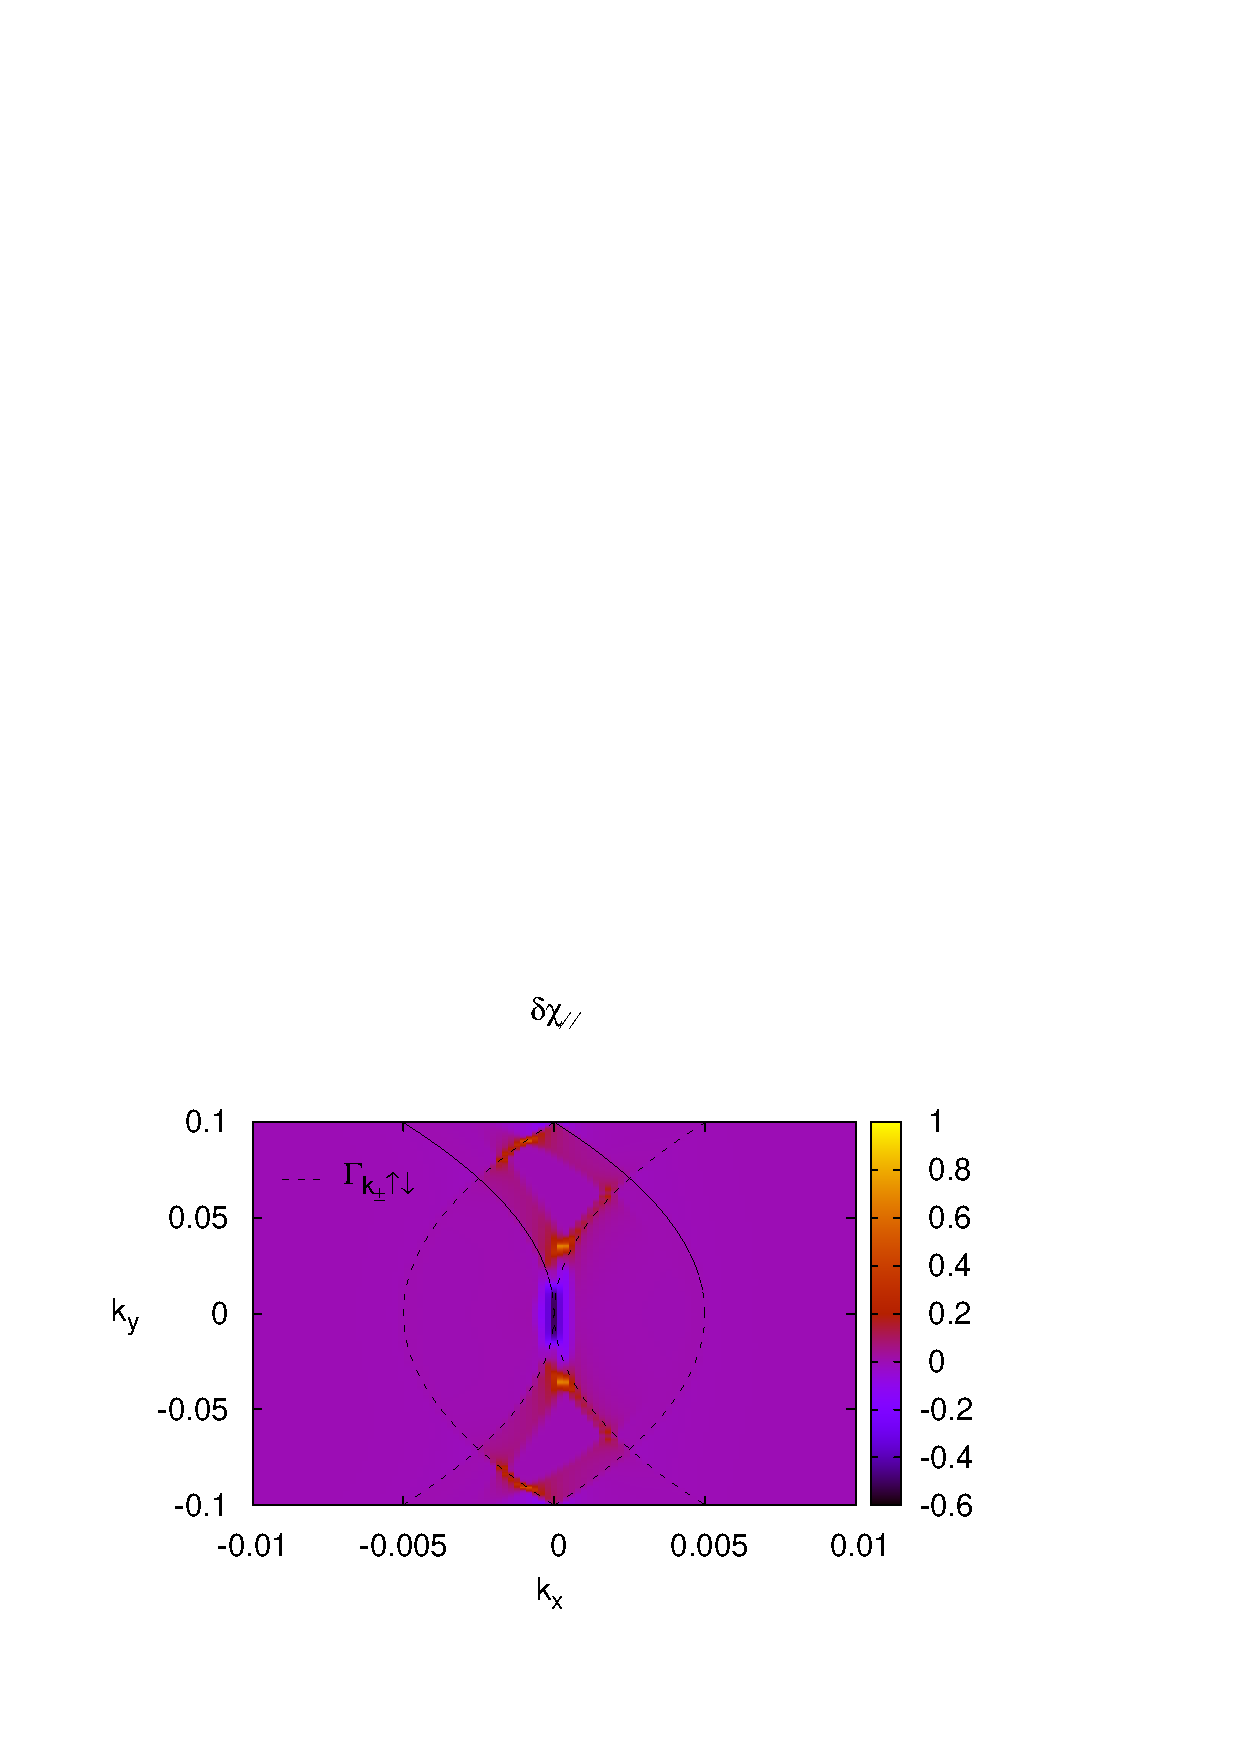
\includegraphics[scale=0.41]{Integrand_zz.jpg}    
	\end{column}
  \end{columns}
\begin{center}
{\Fontvi $T=0.005T_c$, $\mu_e H=0.48\Delta_0$, $\Delta_0=0.01\epsilon_f$, Background$\approx 10^{-3}-10^{-4}$}
\end{center}
\end{frame}


%%%%%%%%%%%%%%%%%%%%%%%
\begin{frame} \frametitle{Calculation}
{\Fontb \textcolor{red}{GOAL}:Maximize $\chi^{sc}$ at given T and H by varying {\bf q}\\
$\delta \chi \propto$1/(Excitation Energies){\Fontvi $\quad \epsilon_{ks}=\sqrt{\Delta_k^2+\xi_k^2}+s\mu_eH$}\\
\colorbox{purple}{\textcolor{yellow}{$\epsilon_{k_-s}=\epsilon_{k_+s}=0$}}
 $\Rightarrow$\fbox{\textcolor{blue}{$\mu_e H$}$=\Delta_{T,H} \sin 2\theta_k^*$}}

\vspace{0.5cm}
 \begin{columns}
    \begin{column}{0.5\textwidth}
      \centering
      $\hat{\bf q}$=nodal direction \\
 	-Maximizes $\chi^{sc}_{\perp}$ \\
        \includegraphics[scale=0.23]{fermiHotSpotsxx3.jpg}
      \end{column}
    \begin{column}{0.5\textwidth}\centering	
	$\hat{\bf q}$=off nodal direction \\
	-Maximizes $\chi^{sc}_{\parallel}$ \\
      \includegraphics[scale=0.23]{fermiHotSpotszz3.jpg}
	\end{column}
  \end{columns}
\end{frame}


%\begin{frame} \frametitle{Calculation}
% \begin{columns}
%    \begin{column}{0.5\textwidth}
%      \centering
%	\includegraphics[scale=0.45]{fermiHotSpotsxx1.eps} \\
%	\includegraphics[scale=0.45]{fermiHotSpotsxx2.eps} \\
%	\includegraphics[scale=0.45]{fermiHotSpotsxx3.eps} \\
%      \end{column}
%    \begin{column}{0.5\textwidth}\centering	
%    \includegraphics[scale=0.45]{fermiHotSpotszz1.eps} \\ 
%      \includegraphics[scale=0.45]{fermiHotSpotszz2.eps}    \\
%      \includegraphics[scale=0.45]{fermiHotSpotszz3.eps}  \\
%	\end{column}
%  \end{columns}
% {\Fontvi Both $q^*$'s are decreasing functions of H}
%\end{frame}
%%%%%%%%%%%%%%%%%%%%%%%%%



\begin{frame}\frametitle{Results}

 \begin{columns}
    \begin{column}{0.5\textwidth} 
	\centering \colorbox{yellow}{\textcolor{black}{$max_{{\bf q}}(\delta\chi_{\perp})=max_{{\bf q}}(\chi^{sc}_{\perp})$}}
            \end{column}
    \begin{column}{0.5\textwidth}   
    \centering \colorbox{yellow}{\textcolor{black}{Two possible maxima?}}
   	\end{column}
  \end{columns}
  \centering{\Fontvii $T=0.005T_c, \quad\mu_e H=0.5\Delta_0, \quad\Delta_0=0.01\epsilon_f$}
 \begin{columns}
    \begin{column}{0.5\textwidth} 
	\includegraphics[height=0.5\textwidth,width=\textwidth]{enh_qqx0.eps}
            \end{column}
    \begin{column}{0.5\textwidth} 
	\includegraphics[height=0.5\textwidth,width=\textwidth]{enh_qqz0.eps} 
   	\end{column}
  \end{columns}
\centering{\Fontvii $T=0.05T_c, \quad\mu_e H=0.5\Delta_0, \quad\Delta_0=0.01\epsilon_f$}
 \begin{columns}
    \begin{column}{0.5\textwidth} 
	\includegraphics[height=0.5\textwidth,width=\textwidth]{enh_qqx1.eps}
            \end{column}
    \begin{column}{0.5\textwidth}	
    	\includegraphics[height=0.5\textwidth,width=\textwidth]{enh_qqz1.eps}
   	\end{column}
  \end{columns}
\end{frame}


\begin{frame}\frametitle{Results}
\centering {\bf \% Enhancement} {\Fontvi $\mathcal{O}(\Delta/\epsilon_f)$}, $\Delta_0=0.005\epsilon_f$,\\
\includegraphics[height=0.6\textwidth,width=\textwidth]{maxsus_diagram.pdf}
\end{frame}
\begin{frame}\frametitle{Results}
\centering {\bf \% Enhancement} {\Fontvi $\mathcal{O}(\Delta/\epsilon_f)$}, $\Delta_0=0.005\epsilon_f$,\\
\includegraphics[height=0.6\textwidth,width=\textwidth]{maxsus_diagram2.jpg}
\end{frame}

\begin{frame}\frametitle{Conclusions}
-Magnetic susceptibility in superconducting state can be enhanced compared to the normal state in high uniform magnetic fields \\
\hspace{0.5cm}{\Fontvi-This may promote AF order with ${\bf q}=2k_f-\delta$ inside SC state}\\[0.5cm]
-Both $\chi_{\parallel}$ and $\chi_{\perp}$ show enhancement ($\perp$ in CeCoIn$_5$) \\[0.5cm]
-$\chi^{sc}$ contours qualitatively align with Q-phase boundary\\{\Fontvii(Kenzelmann et al, Phys. Rev. Lett. (2010). Kato et al, Phys. Rev. Lett. (2011))} \\[0.5cm]
-Connection to order parameter:\\
{\Fontvi
\hspace{0.5cm}-No enhancement seen for S-wave \\
\hspace{0.5cm}-$\perp$ enhancement requires sign changing (nodal) order parameter \\
\hspace{0.5cm}-$\parallel$ enhancement requires sufficiently small minimum in order parameter\\
\hspace{0.5cm}-Possible tool to determine near nodal direction}
 \end{frame}

%\begin{frame}\frametitle{}
%\begin{center}
%{\Fontb Thank You!} \\[2cm]
%{\Fontb Questions?}
%\end{center}
%\end{frame}

\begin{frame}
Normal state Susceptibility \\[1cm]
${\Fontvii\frac{\chi^N_\parallel(q)}{\chi^N_0} = \left\{
     \begin{array}{lr}
       1: \quad q < 2\sqrt{1-\mu_e H/\epsilon_f}\\
       1-\frac{1}{2}\sqrt{1-(\frac{2}{q})^2(1-\mu_e H/\epsilon_f)}: \quad q \in [2\sqrt{1-\mu_e H/\epsilon_f},2\sqrt{1+\mu_e H/\epsilon_f}] \\
       1-\frac{1}{2}\sqrt{1-(\frac{2}{q})^2(1-\mu_e H/\epsilon_f)}-\frac{1}{2}\sqrt{1-(\frac{2}{q})^2(1+\mu_e H/\epsilon_f)}: q > 2\sqrt{1+\mu_e H/\epsilon_f}
     \end{array}
   \right. }$ \\[1cm]
${\Fontvii\frac{\chi^N_\perp(q)}{\chi^N_0} = \left\{
     \begin{array}{lr}
       1 :\quad q < \sqrt{1-\mu_e H/\epsilon_f}+\sqrt{1+\mu_e H/\epsilon_f} \\
       1-\sqrt{1-(\frac{2}{q})^2+(\frac{2\mu_e H/\epsilon_f}{q^2})^2} : \quad q >\sqrt{1-\mu_e H/\epsilon_f}+\sqrt{1+\mu_e H/\epsilon_f}
     \end{array}
   \right.}$
   
    \begin{columns}
    \begin{column}{0.5\textwidth}
      \centering
      \textcolor{red}{\bf Maximize $\delta\chi^{sc}_{\perp}$} \\
      $\hat{\bf q}$=nodal direction \\
	 $\Delta({\bf k})=\Delta_{T,H}\sin({2\theta_k})$ \\
        $q^*=\sqrt{2(1+\sqrt{1-\bigg(\frac{\mu_eH}{\Delta_{T,B}}\bigg)^2}}\hat{x}$
      \end{column}
    \begin{column}{0.5\textwidth}\centering	
	\textcolor{red}{\bf Maximize $\delta\chi^{sc}_{\parallel}$} \\
	$\hat{\bf q}$=off nodal direction \\
     	$\Delta({\bf k})=\Delta_{T,H}\cos({2\theta_k +\eta_{q^*}})$ \\
        $q^*\approx2\sqrt{1-\frac{\mu_eH}{\epsilon_f}}+\delta\hspace{0.2cm}\hat{x}$
        {\Fontvii$\eta_{q^*}\approx\sin^{-1}\frac{\mu_e H}{\Delta_{T,B}}-\sin^{-1}\bigg(\sqrt{1-\big(\frac{q^*}{2\sqrt{1+\mu_eH/\epsilon_f}}\big)^2}\bigg)$}   \\
	\end{column}
  \end{columns}
\end{frame}

\end{document}